\documentclass[12pt]{article}

\usepackage{titling}
\usepackage{caption}
\usepackage{multirow}
\usepackage[T1]{fontenc}
\usepackage[utf8]{inputenc}
\usepackage[italian]{babel}
\usepackage{tabularx}
\usepackage [colorlinks=true,urlcolor=blue, linkcolor=black]{hyperref}
\newcommand{\subtitle}[1]{%
  \posttitle{%
    \par\end{center}
    \begin{center}\LARGE#1\end{center}
    \vskip0.5em}%
}

\setlength{\oddsidemargin}{0in}
\setlength{\evensidemargin}{0in}
\setlength{\topmargin}{0in}
\setlength{\headsep}{-.25in}
\setlength{\textwidth}{6.5in}
\setlength{\textheight}{8.5in}

\font\myfont=cmr12 at 40pt

\usepackage{eurosym}
\newcommand{\pedice}{\ped { \textbf{G}}}
\title{\myfont{Analisi dei requisiti}}
\author{Dream Corp.}

\date{ \myfont 05-12-2018}


\begin{document}
	\maketitle
	\begin{center}
	\huge Versione 1.0.0
	\\G\&B
	\end{center}
	\newpage
	
		\section{Log delle Modifiche}
Di seguito viene presentata una tabella riportante le modifiche al file "Analisi dei requisiti".

\begin{table}[!h] % h! serve per posizionarla relativamente
            \centering
            \renewcommand{\arraystretch}{2}
            \rowcolors{2}{gray!25}{white} %colori alternati, grigio 25% e bianco 100%
            \begin{tabular}{|c|c|p{5cm}|c|c|} % p{dimensione desiderata}
                \rowcolor{orange!50} %colore intestazione
        		\hline
        		\textbf{Versione} & \textbf{Data} & \textbf{Descrizione} & \textbf{Autore} & \textbf{Ruolo} \\
                \hline
                1.0.0 & 9/01/2019 & Approvazione documento per rilascio RR & Pietro Casarotto & Responsabile \\
                \hline
                0.1.0 & 8/01/2019 & Superamento verifica & Gianluca Pegoraro & Verificatore \\
                \hline
                0.0.22 & 6/01/2018 & Correzione casi d’uso & Matteo Bordin & Analista \\
                \hline
                0.0.21 & 5/01/2019 & Correzione paragrafo §6.2 & Davide Liu & Analista \\
                \hline
                0.0.20 & 4/01/2019 & Richiesta di modifica dei casi d’uso UC2 e UC6 e contenuto tabelle paragrafi §6.1 e §6.2 & Gianluca Pegoraro & Verificatore \\
                \hline
                0.0.19 & 2/01/2019 & Stesura paragrafo §7 & Davide Ghiotto & Analista \\
                \hline
                0.0.18 & 2/01/2019 & Conclusione paragrafo §6.2 & Davide Ghiotto & Analista \\
                \hline
                0.0.17 & 30/12/2018 & Continuazione paragrafo §6.2 & Davide Liu & Analista \\
                \hline
                0.0.16 & 30/12/2018 & Stesura paragrafo §6.1 & Davide Liu & Analista \\
                \hline
                0.0.15 & 30/12/2018 & Conclusione stesura diagrammi UML dei casi d’uso paragrafo §5 & Matteo Bordin & Analista \\
                \hline
                0.0.14 & 28/12/2018 & Inizio stesura diagrammi UML dei casi d'uso paragrafo §5 & Matteo Bordin & Analista \\
                \hline
                0.0.13 & 28/12/2018 & Inizio paragrafo §6.2 & Davide Ghiotto & Analista \\
                \hline
                
        \end{tabular}
        \caption{Log delle Modifiche} %descrizone a fine tabella
        \label{tab:Log delle modifiche}
\end{table}

\begin{table}[h!] % h! serve per posizionarla relativamente
            \centering
            \renewcommand{\arraystretch}{2}
            \rowcolors{2}{gray!25}{white} %colori alternati, grigio 25% e bianco 100%
            \begin{tabular}{|c|c|p{5cm}|c|c|} % p{dimensione desiderata}
                \rowcolor{orange!50} %colore intestazione
        		\hline
        		\textbf{Versione} & \textbf{Data} & \textbf{Descrizione} & \textbf{Autore} & \textbf{Ruolo} \\
                \hline
                0.0.12 & 22/12/2018 & Aggiunta casi d’uso UC9, UC10 & Matteo Bordin & Analista \\
                \hline
                0.0.11 & 21/12/2018 & Correzione struttura casi d’uso paragrafo §5 & Davide Liu & Analista \\
                \hline
                0.0.10 & 20/12/2018 & Aggiunta casi d’uso UC6, UC7, UC8 & Davide Ghiotto & Analista \\
                \hline
                0.0.9 & 19/12/2018 & Modifica caso d’uso UC1 & Matteo Bordin & Analista \\
                \hline
                0.0.8 & 19/12/2018 & Aggiunta casi e sotto casi d’uso UC3, UC5 & Matteo Bordin & Analista \\
                \hline
                0.0.7 & 18/12/2018 & Aggiunta casi d’uso UC1, UC2, UC4 & Davide Ghiotto & Analista \\
                \hline
                0.0.6 & 17/12/2018 & Stesura paragrafo §5.1, §5.2 & Davide Liu & Analista \\
                \hline
                0.0.5 & 16/12/2018 & Stesura paragrafo §4 & Matteo Bordin & Analista \\
                \hline
                0.0.4 & 16/12/2018 & Stesura paragrafo §3 & Davide Liu & Analista \\
                \hline
                0.0.3 & 16/12/2018 & Sistemazione  paragrafo §2.4 & Davide Ghiotto & Analista \\
                \hline 
                0.0.2 & 14/12/2018 & Stesura introduzione paragrafo §2 & Davide Liu & Analista \\
                \hline
                0.0.1 & 10/12/2018 & Creazione scheletro del documento & Davide Liu & Analista \\
                \hline
                
                
                
                
        \end{tabular}
        \caption{Log delle Modifiche} %descrizone a fine tabella
        \label{tab:Log delle modifiche2}
\end{table}

	
	\newpage
	\tableofcontents
	\newpage
	
	\section{Introduzione}
		\subsection{Scopo del documento}			
Questo documento si pone come obiettivo quello di effettuare un' analisi dei requisiti per la progettazione e lo sviluppo del capitolato(G) "G\&B: monitoraggio intelligente di processi DevOps" (Capitolato C3) proposto dall'azienda Zucchetti.


		\subsection{Obiettivo del prodotto}

Il sistema da realizzare sarà  un plug-in di Grafana(G), scritto in linguaggio JavaScript(G), che leggerà da un file json(G) contenente la definizione della rete Bayesiana(G) e quindi permetterà di associare ad alcuni nodi della rete data un flusso di monitoraggio.
Ad intervalli predefiniti, verranno eseguiti i calcoli previsti dalla rete Bayesiana, modificando le probabilità dei nodi derivati in base ai dati rilevati dal campo.


		\subsection{Note esplicative}

Allo scopo di evitare ambiguità a lettori esterni al gruppo, si specifica che all'interno del documento verranno inseriti dei termini con un carattere g come pedice, questo significa che il significato inteso in quella situazione è stato inserito nel Glossario.


		\subsection{Riferimenti }

		\subsubsection{Riferimenti Normativi}
		\begin{itemize}
			\item Norme di progetto v 1.0.0
			\item Capitolato C3: G\&B: monitoraggio intelligente di processi DevOps.\newline
			\url{https://www.math.unipd.it/~tullio/IS-1/2018/Progetto/C3.pdf}
			\item Grafana:\newline
			\url{https://grafana.com/}
			\item Libreria Open Source per reti bayesiane:\newline
			\url{https://github.com/vangj/jsbayes}
			\item Slide lezioni utilizzate durante il corso di Ingegneria del Software:\newline
			\url{https://www.math.unipd.it/~tullio/IS-1/2018/}
		\end{itemize}

		\subsubsection{Riferimenti Informativi}
			\begin{itemize}
			\item Piano di qualifica v 1.0.0
			\item Slide del corso di "Ingegneria del Software"\newline
			\url{https://www.math.unipd.it/~tullio/IS-1/2018/}
		\end{itemize}
				

\newpage

	
	\section{Descrizione prodotto}
		\subsection{Scopo del prodotto}			
Si devono realizzare dei sistemi che possano applicare metodi di intelligenza artificiale\pedice al flusso dei dati raccolti, al fine non solo di monitorare la situazione del sistema ma anche per consigliare gli interventi o quanto meno le zone di intervento alla linea di produzione del software.
Il presente capitolato ha per oggetto l'affidamento della fornitura per la
realizzazione di un plugin per lo strumento di monitoraggio Grafana\pedice che
applichi reti Bayesiane\pedice al flusso dei dati ricevuti per allarmi o segnalazioni tra gli operatori del servizio Cloud e la linea di produzione del software.


		\subsection{Funzioni del prodotto}
Il plugin deve poter leggere la definizione di una rete Bayesiana da un file in formato json. Avverrà successivamente l'associazione dei flussi di monitoraggio con i nodi della rete Bayesiana inserita. I nodi della rete mapperanno gli stati dei flussi di monitoraggio e il cambio di stato avverrà nel momento in cui si rileverà una variazione di valore nel flusso dati. Questa variazione del valore verrà catturata dal sistema di Grafana, dopo la definizione di un alert opportuno per quel flusso di monitoraggio. Un alert è un messaggio che viene inviato da Grafana, riportante lo stato del nodo monitorato e il suo valore, quando quest'ultimo viola una delle condizioni poste. L'alert può essere modificato e rimosso a discrezione dell'utente.
Nel momento in cui un alert viene lanciato il sistema avvia il ricalcolo delle probabilità dell'intera rete grazie al supporto della libreria jsbayes. 
I valori ricalcolati delle probabilità dei nodi della rete a cui non è stato associato un flusso di monitoraggio verranno rappresentati con dei grafici, detti "panel", grazie al supporto di Grafana.
Su questi valori probabilistici verranno a loro volta applicati opzionalmente degli alert, i quali si attiveranno quando le stime su queste percentuali supereranno una certa soglia decisa dall'utente.


		\subsection{Tipologia di utenti}

Il prodotto è rivolto a tutti coloro che gestiscono i sistemi di raccolta e collezione di dati in modo da poterli monitorare ed intervenire qualora sia necessario, grazie a degli allarmi forniti dal plugin.
Gli utenti devono avere familiarità  con il tool di monitoraggio Grafana.


		\subsection{Vincoli di progettazione}
			\subsubsection{Requisiti obbligatori}
				\begin{itemize}
					\item Leggere la definizione della rete Bayesiana da un file in formato json;
					\item Associare i nodi della rete, letta dal file json, ad un flusso di dati presente in Grafana;
					\item Applicare il ricalcolo delle probabilità della rete secondo regole temporali prestabilite;
					\item Fornire nuovi dati al sistema di Grafana derivati dai nodi della rete non collegati al flusso di monitoraggio;
					\item Rendere disponibili i dati al sistema di creazione di grafici e dashboard per la loro visualizzazione.
		        	\end{itemize}
			\subsubsection{Requisiti opzionali}
				\begin{itemize}
					\item Possibilità di definire "alert\pedice" in base a livelli di soglia raggiunti dai nodi non collegati al flusso dei dati;
					\item Possibilità di disegnare la rete Bayesiana con un piccolo editor grafico specializzato;
					\item Possibilità di applicare più reti Bayesiane in oggetti di monitoraggio diversi;
					\item Possibilità di creare una rete Bayesiana a partire dai dati raccolti sul campo anziché svilupparla con la collaborazione degli esperti del settore;
					\item Identificare altri metodi di Intelligenza Artificiale oltre alla rete Bayesiana che siano applicabili all'analisi del flusso di dati di monitoraggio.
		        	\end{itemize}
		        \subsubsection{Requisiti opzionali scelti da implementare}
				\begin{itemize}
					\item Possibilità di definire "alert" in base a livelli di soglia raggiunti dai nodi non collegati al flusso dei dati;
					\item Possibilità di applicare più reti Bayesiane in oggetti di monitoraggio diversi.
	        		\end{itemize}
				
				
			\subsection{Vincoli generali}			
Essendo il prodotto un plugin per Grafana (versione 5.4.3), occorre aver scaricato e configurato Grafana (versione 5.4.3 o superiore) in modo da poter installare il plugin.

	\section{Grafana e reti Bayesiane}
		\subsection{Grafana}			
Grafana è uno strumento di monitoraggio\pedice dati open-source, tramite delle dashboard è possibile visualizzare e tenere sottocontrollo i risultati delle query\pedice loro associate e lanciare un allarme in caso di superamento di valori soglia prestabiliti dall'utente. E' molto utilizzato dalle aziende per via delle sue molteplici funzionalità  espandibili tramite vari plug-in sviluppati dagli utenti.


		\subsection{Reti Bayesiane}
Una Rete Bayesiana è un grafo, ossia un'insieme di nodi e frecce. I nodi
indicano le variabili di un problema in gioco, mentre le frecce indicano i
rapporti di causalità tra di esse e costituiscono un potente mezzo per
modellizzare un problema ed esprimere i rapporti tra le grandezze in gioco.
Ad una rete bayesiana possono essere fornite delle "evidenze", ossia valori noti di variabili del problema. 
La rete calcola come la conoscenza di queste variabili modifica la probabilità  delle altre variabili.
Anche se non si ha idea di quali siano i rapporti di mutua dipendenza tra
variabili, gli algoritmi di "structure learning" riescono a ricostruire la corretta struttura della rete, sempre che si abbia a disposizione un adeguata base dati.
Sostanzialmente le Reti Bayesiane possono essere utilizzate come potenti mezzi
di "machine learning\pedice". Esse riescono ad individuare i fattori decisivi che
determinano i valori di una variabile, individuare la categoria cui appartengono determinate osservazioni e prevedere comportamenti futuri in base all'esperienza di quelli passati.


\newpage


	\section{Casi d'Uso}
		\subsection{Attori}
			I casi d'uso definiscono interazioni tra il sistema e gli attori esterni. L'elenco di questi ultimi e l'analisi delle relazioni in funzione dei diversi scopi che questi attori perseguono è fondamentale per una corretta descrizione dei casi d'uso.
        Riportiamo due attori:
        \begin{itemize}
            \item Utente generico;
            \item Grafana.
        \end{itemize}

		\subsection{Tracciamento Casi d'Uso}
        Al fine di classificare e rendere leggibili i casi d'uso abbiamo deciso di utilizzare una codifica per descriverli. Ad ogni caso d'uso verrà quindi associata una stringa univoca strutturata nel seguente modo:
        \begin{equation}
            UCX.Y.Z    
        \end{equation}
        dove X,Y,Z sono dei numeri progressivi per indicare specificità all'interno dei casi d'uso. \newline
        \newline
        Per rappresentare una scelta tra casi d'uso tra loro mutuamente esclusivi abbiamo deciso di adottare il seguente criterio: nella codifica del caso d'uso verrà aggiunta una lettera maiuscola, tra parentesi tonde, per indicare un insieme di scelte per risolvere il caso d'uso generico, rappresentato dalla normale codifica numerica X.Y.Z. La finale codifica di un caso d'uso di specializzazione sarà quindi:
        \begin{equation}
            UCX(A).Y(A).Z(A)
        \end{equation}
        L'utilizzo di tale criterio sarà utilizzato solo in caso di bisogno e quindi non è detto che sia presente in tutti i casi d'uso.
        
 
        \begin{figure}[!htbp]
                	\centering
                	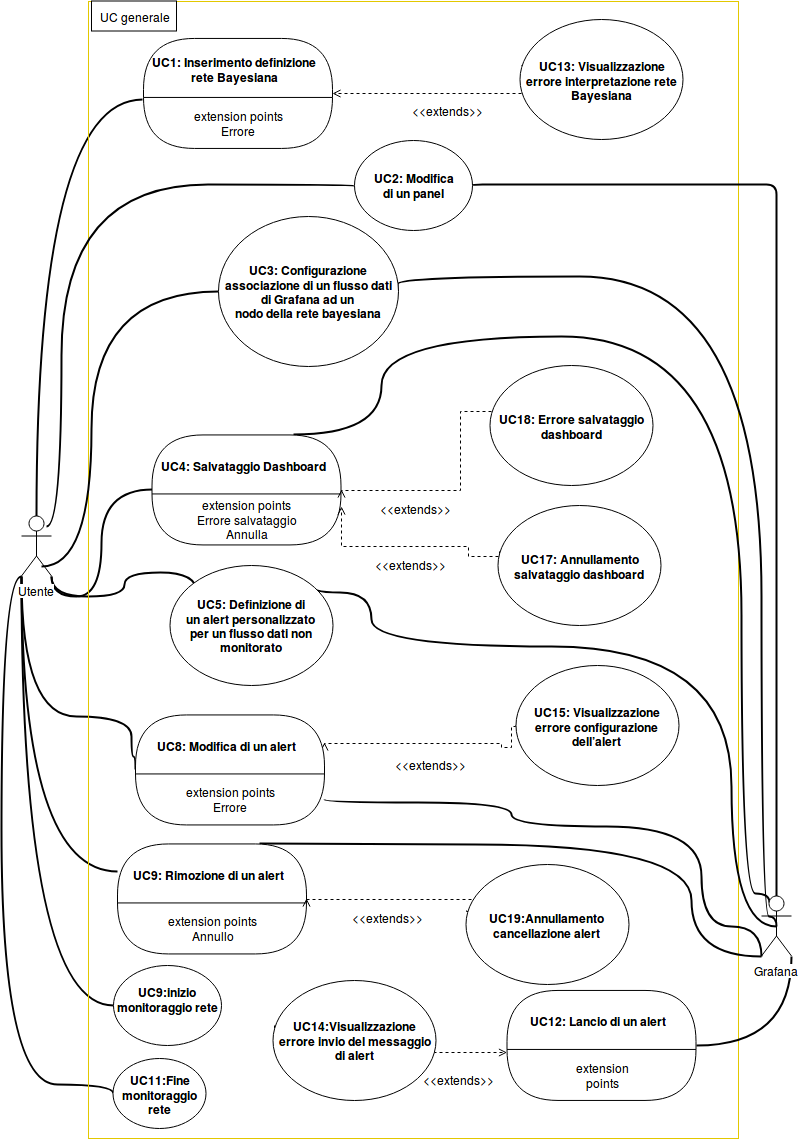
\includegraphics[width=\textwidth]{UCgeneral.png}
                	\caption{UCgenerale: Caso d'uso generale}
                \end{figure}  
              \clearpage      
		\subsection{Attore primario: Utente generico}
		Si riferiscono a tutti quei casi d'uso che hanno come attore primario l'utente e come attore secondario Grafana. Descrivono tutte le interazioni possibili compiute direttamente dall'utente.
                    
                        
		
				\subsubsection{UC1: Inserimento definizione rete Bayesiana}
                    \textbf{Precondizione:} L’utente deve trovarsi nell'interfaccia principale e deve possedere una definizione di rete Bayesiana che vuole inserire (Fig.\ref{uc1}).
                    \newline
                    \textbf{Postcondizione:} Viene inserita nell'applicativo la definizione di rete.
                    \newline
                    \textbf{Attore primario:} Utente.
                    \newline
                    \textbf{Contestualizzazione / Scenario principale:} L’utente carica la definizione della rete Bayesiana.
                    \newline
                    \textbf{Estensioni:} 
                    	\begin{enumerate}
                            \item Problema con l’interpretazione della rete Bayesiana \underline{\textit{UC11}}.
                        \end{enumerate}
                        
                    \begin{figure}[!htbp]
                    	\centering
                    	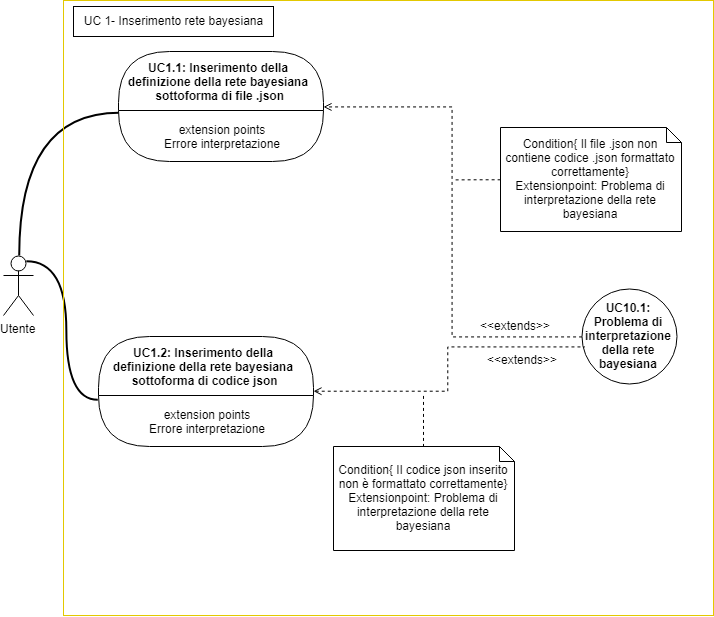
\includegraphics[scale=0.55]{UC1.png}
                    	\caption{UC1: Inserimento definizione rete Bayesiana}
                    	\label{uc1}
                    \end{figure}
                    \clearpage
                
                        
                \subsubsection{UC1(A): Inserimento definizione della rete bayesiana sotto forma di file json}
                    \textbf{Descrizione:} L’utente vuole inserire la definizione della rete bayesiana sotto forma di file json.\\
                    \textbf{Precondizione:}  L’utente deve trovarsi nell'interfaccia principale e possedere un file json contenente una definizione di rete Bayesiana che vuole inserire (Fig.\ref{uc1a}).
                    \newline
                    \textbf{Postcondizione:} Viene inserita nell'applicativo la definizione di rete presente nel file json.
                    \newline
                    \textbf{Attore primario:} Utente.
                    \newline
                    \textbf{Contestualizzazione / Scenario principale:} \begin{enumerate}
                        \item L’utente preme il pulsante per l’upload del file json contenente la definizione di rete;
                        \item L’utente sceglie il file \underline{\textit{UC1(A).1}};
                        \item Upload del file;
                        \item La rete viene caricata.
                    \end{enumerate}
                    
                    \textbf{Estensioni:} \begin{enumerate}
                            \item C’è stato un problema con l’interpretazione della rete Bayesiana \underline{\textit{UC11}}.
                        \end{enumerate}
                        
                    \begin{figure}[!htbp]
                    	\centering
                    	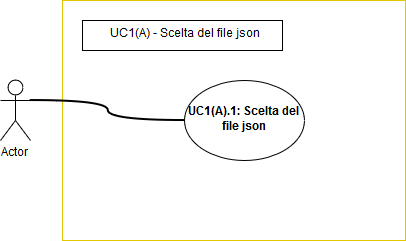
\includegraphics[scale=0.8]{UC1(A).png}
                    	\caption{UC1(A): Inserimento definizione della rete bayesiana sotto forma di file json}
                    	\label{uc1a}
                    \end{figure}
                    
                    \clearpage    
                    
                \subsubsection{UC1(A).1: Scelta del file json }
                     \textbf{Descrizione:} L’utente sceglie il file json.\\
                    \textbf{Precondizione:} È disponibile la schermata di selezione del file.   
                    \newline
                    \textbf{Postcondizione:} Il file è stato selezionato. 
                    \newline
                    \textbf{Attore primario:} Utente.
                    \newline
                    \textbf{Contestualizzazione / Scenario principale:} \begin{enumerate}
                        \item L’utente sceglie il file.
                    \end{enumerate}
                    
                        
                \subsubsection{UC1(B): Inserimento definizione rete Bayesiana sotto forma di codice json}
                    \textbf{Descrizione:} L’utente vuole inserire la definizione della rete bayesiana sotto forma di codice json.\\
                    \textbf{Precondizione:}  L’utente deve trovarsi nell'interfaccia principale di Grafana e possedere codice json di una definizione di rete Bayesiana che vuole inserire.
                    \newline
                    \textbf{Postcondizione:} Viene inserita nell'applicativo la definizione di rete descritta dal codice json.
                    \newline
                    \textbf{Attore primario:} Utente.
                    \newline
                    \textbf{Contestualizzazione / Scenario principale:} \begin{enumerate}
                        \item L’utente incolla il codice json nel text area dedicata;
                        \item L’utente preme il pulsante “Insert Bayesian Network”;
                        \item La rete viene caricata.
                    \end{enumerate}
                    
                    \textbf{Estensioni:} \begin{enumerate}
                            \item C’è stato un problema con l’interpretazione della rete bayesiana \underline{\textit{UC11}}.
                        \end{enumerate}
                        
                
                        
                \subsubsection{UC2: Modifica di un panel}
                    \textbf{Descrizione:} L’utente vuole modificare delle impostazioni di un determinato panel (Fig.\ref{uc2}).
                    \newline
                    \textbf{Precondizione:} Deve essere presente almeno un flusso dati rappresentato da un panel.
                    \newline
                    \textbf{Postcondizione:} Il panel selezionato è stato modificato.
                    \newline
                    \textbf{Attore primario:} Utente.
                    \newline
                    \textbf{Attore secondario:} Grafana.
                    \newline
                    \textbf{Contestualizzazione / Scenario principale:} \begin{enumerate}
                        \item L’utente seleziona un flusso dati di monitoraggio \underline{\textit{UC2.1}};
                        \item L’utente entra in modalità "modifica" del flusso dati selezionato \underline{\textit{UC2.2}};
                        \item L’utente modifica le informazioni principali del panel \underline{\textit{UC2.3}};
                        \item L’utente è soddisfatto delle modifiche;
                        \item L'utente salva le modifiche, salvando la dashboard \underline{\textit{UC4}}.
                        \item L’utente chiude la modalità "modifica" del panel \underline{\textit{UC2.4}}.
                    \end{enumerate}
                    
                    \begin{figure}[!htbp]
                    	\centering
                    	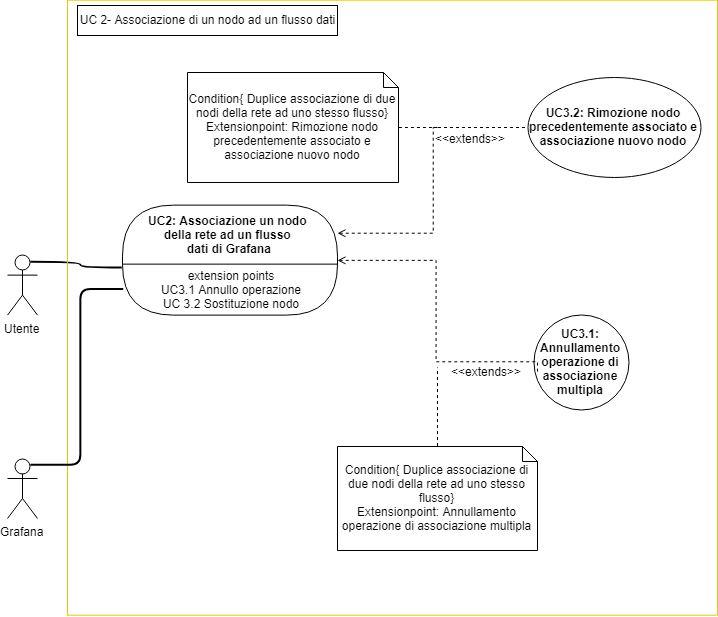
\includegraphics[scale=0.6]{UC2.png}
                    	\caption{UC2: Modifica di un panel}
                    	\label{uc2}
                    \end{figure}
                    \clearpage
                \subsubsection{UC2.1: Selezione del flusso di monitoraggio}
                    \textbf{Descrizione:} L'utente seleziona il panel che monitora i dati del flusso di interesse.\\
                    \textbf{Precondizione:} L'utente deve possedere un flusso dati rappresentato da un panel.
                    \newline
                    \textbf{Postcondizione:} Un flusso di monitoraggio è selezionato, facendo comparire delle operazioni possibili su di esso.
                    \newline
                    \textbf{Attore primario:} Utente.
                    \newline
                    \textbf{Contestualizzazione / Scenario principale:} \begin{enumerate}
                        \item L’utente seleziona, tra i diversi panel nella sua dashboard, quello che rappresenta graficamente il flusso dati di interesse e preme sul titolo.
                    \end{enumerate}
                    
                \subsubsection{UC2.2: Attivazione modalità "modifica" di un panel}
                    \textbf{Descrizione:} L'utente attiva la modalità "modifica" di un panel.
                    \newline
                    \textbf{Precondizione:} L'utente deve aver selezionato un flusso dati premendo sul titolo del panel relativo.
                    \newline
                    \textbf{Postcondizione:} Un flusso di monitoraggio è in modalità "modifica".
                    \newline
                    \textbf{Attore primario:} Utente.
                    \newline
                    \textbf{Contestualizzazione / Scenario principale:} \begin{enumerate}
                        \item L’utente sceglie la funzione "Edit" tra le opzioni eseguibili.
                    \end{enumerate}
                    
                    
                    
                \subsubsection{UC2.3:  Modifica delle informazioni principali di un panel}
                    \textbf{Descrizione:} L’utente modifica le informazioni generali del panel inserendo titolo e descrizione (Fig.\ref{uc2.3}).
                    \newline
                    \textbf{Precondizione:} L'utente deve trovarsi in modalità "modifica" di un panel.
                    \newline
                    \textbf{Postcondizione:} Vengono modificate delle informazioni del panel interessato.
                    \newline
                    \textbf{Attore primario:} Utente.
                    \newline
                    \textbf{Contestualizzazione / Scenario principale:} \begin{enumerate}
                        \item L'utente seleziona la sezione "General" all'interno della schermata di modifica del panel;
                        \item L’utente modifica il titolo \underline{\textit{UC2.3.1}};
                        \item L’utente modifica la descrizione \underline{\textit{UC2.3.2}};
                        \item L'utente salva la dashboard \underline{\textit{UC4}}.
                    \end{enumerate}
                    
                    \begin{figure}[!htbp]
                    	\centering
                    	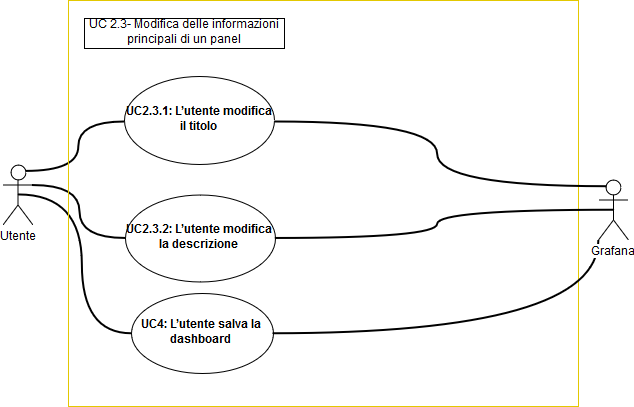
\includegraphics[width=\textwidth]{UC2-3.png}
                    	\caption{UC2.3:  Modifica delle informazioni principali di un panel}
                    	\label{uc2.3}
                    \end{figure}
                    
                \subsubsection{UC2.3.1: Modifica titolo di un panel}
                    \textbf{Descrizione:} L’utente modifica il titolo per meglio identificare il flusso dati rappresentato.
                    \newline
                    \textbf{Precondizione:} L'utente deve trovarsi in modalità "modifica" di un panel e essere nella sezione "General".
                    \newline
                    \textbf{Postcondizione:} Viene modificato il titolo del panel.
                    \newline
                    \textbf{Attore primario:} Utente.
                    \newline
                    \textbf{Contestualizzazione / Scenario principale:} \begin{enumerate}
                        \item L’utente modifica il titolo a piacimento nell'apposita sezione "Title".
                    \end{enumerate}
                
                \subsubsection{UC2.3.2: Modifica descrizione di un panel}
                    \textbf{Descrizione:} L’utente modifica la descrizione per permettere una più completa comprensione del flusso dati rappresentato.
                    \newline
                    \textbf{Precondizione:} L'utente deve trovarsi in modalità "modifica" di un panel e essere nella sezione "General".
                    \newline
                    \textbf{Postcondizione:} Viene modificata la descrizione del panel.
                    \newline
                    \textbf{Attore primario:} Utente.
                    \newline
                    \textbf{Contestualizzazione / Scenario principale:} \begin{enumerate}
                        \item L’utente modifica la descrizione a piacimento nell'apposita sezione "Description".
                    \end{enumerate}
                    
                \subsubsection{UC2.4: Chiusura modalità "modifica" di un panel}
                    \textbf{Descrizione:} L’utente ha terminato le modifiche ed esce dalla modalità "modifica" del panel.
                    \newline
                    \textbf{Precondizione:} L'utente ha salvato la dashboard dopo essere entrato in modalità modifica del panel.
                    \newline
                    \textbf{Postcondizione:} Il panel non è più in modalità "modifica".
                    \newline
                    \textbf{Attore primario:} Utente.
                    \newline
                    \textbf{Contestualizzazione / Scenario principale:} \begin{enumerate}
                        \item L’utente preme la "X" a destra della schermata di modifica del panel.
                    \end{enumerate}
                
    
                        
                \subsubsection{UC3: Configurazione associazione di un flusso dati di Grafana ad un nodo della rete bayesiana}
                    \textbf{Descrizione:} L’utente vuole configurare l'associazione tra il flusso dati rappresentato dal panel selezionato e un nodo di una rete bayesiana per poterci poi applicare metodi di inferenza (Fig.\ref{uc3}).
                    \newline
                    \textbf{Precondizione:} Deve essere presente almeno una definizione di rete bayesiana e l'utente deve trovarsi in modalità "modifica" di un panel.
                    \newline
                    \textbf{Postcondizione:} E' avvenuta la configurazione desiderata dall'utente riguardante l'associazione nodo-flusso dati.
                    \newline
                    \textbf{Attore primario:} Utente.
                    \newline
                    \textbf{Attore secondario:} Grafana.
                    \newline
                    \textbf{Contestualizzazione / Scenario principale:} \begin{enumerate}
                        \item L’utente seleziona la sezione "Bayesian Network" all'interno della schermata di modifica del panel;
                        \item L'utente sceglie la rete bayesiana di interesse da un elenco (se c'è né più di una) \underline{\textit{UC3.1}};
                        \item L'utente modifica l'associazione nodo-flusso dati \underline{\textit{UC3.2}}.
                    \end{enumerate}
                    
                    \begin{figure}[!htbp]
                    	\centering
                    	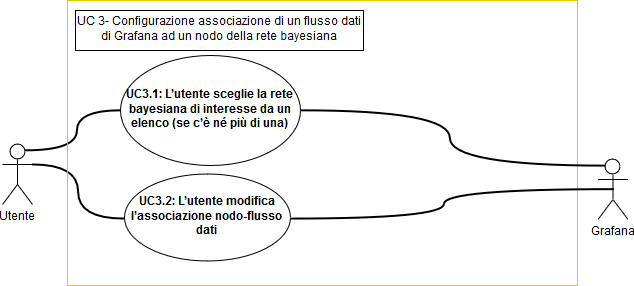
\includegraphics[width=\textwidth]{UC3.png}
                    	\caption{UC3: Configurazione associazione di un flusso dati di Grafana ad un nodo della rete bayesiana}
                    	\label{uc3}
                    \end{figure}
                    
                \subsubsection{UC3.1: Selezione della rete bayesiana}
                    \textbf{Descrizione:} L’utente sceglie, tra le proposte, la rete bayesiana entro cui ricercare il nodo da associare al panel.
                    \newline
                    \textbf{Precondizione:} Il panel è in modalità "modifica".
                    \newline
                    \textbf{Postcondizione:} La rete bayesiana di interesse è selezionata.
                    \newline
                    \textbf{Attore primario:} Utente.
                    \newline
                    \textbf{Attore secondario:} Grafana.
                    \newline
                    \textbf{Contestualizzazione / Scenario principale:} \begin{enumerate}
                        \item L’utente sceglie la rete bayesiana di interesse da un elenco (se c'è né più di una).
                    \end{enumerate}
                    
               
                
                \subsubsection{UC3.2: Modifica associazione nodo-flusso dati}
                    \textbf{Descrizione:} L’utente modifica l'associazione presente, oppure ne crea una nuova, con il flusso dati rappresentato dal panel (Fig.\ref{uc3.2}).
                    \newline
                    \textbf{Precondizione:} L'utente deve aver selezionato un rete bayesiana all'interno della sezione "Bayesian Network" della schermata di modifica di un panel.
                    \newline
                    \textbf{Postcondizione:} Sono state modificate le associazioni nodo-flusso dati.
                    \newline
                    \textbf{Attore primario:} Utente.
                    \newline
                    \textbf{Attore secondario:} Grafana.
                    \newline
                    \textbf{Contestualizzazione / Scenario principale:} \begin{enumerate}
                        \item L’utente modifica l'associazione tra nodi della rete selezionata e il flusso dati rappresentato dal panel in modifica.
                    \end{enumerate}
                    
                     \begin{figure}[!htbp]
                    	\centering
                    	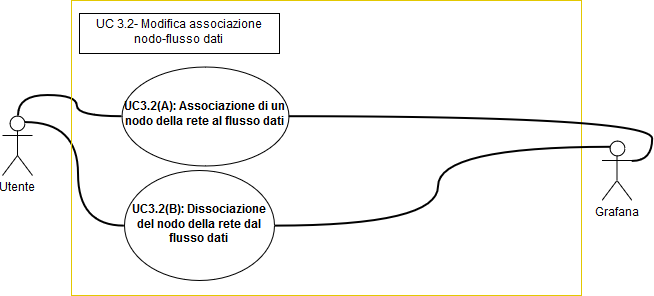
\includegraphics[scale=0.7]{UC3-2.png}
                    	\caption{UC3.2: Modifica associazione nodo-flusso dati}
                    	\label{uc3.2}
                    \end{figure}
                
                \clearpage
                    
                \subsubsection{UC3.2(A): Associazione di un nodo della rete al flusso dati}
                    \textbf{Descrizione:} L’utente sceglie di associare un nodo della rete al flusso dati (Fig.\ref{uc3.2a}).
                    \newline
                    \textbf{Precondizione:} Non è presente un'associazione di un nodo di quella rete con il flusso dati.
                    \newline
                    \textbf{Postcondizione:} E' avvenuta l'associazione del nodo selezionato al flusso dati.
                    \newline
                    \textbf{Attore primario:} Utente.
                    \newline
                    \textbf{Attore secondario:} Grafana.
                    \newline
                    \textbf{Contestualizzazione / Scenario principale:} \begin{enumerate}
                        \item Seleziona il nodo della rete     \underline{\textit{UC3.2(A).1}};
                        \item Seleziona la funzione “Associa” \underline{\textit{UC3.2(A).2}};
                        \item Viene visualizzato un messaggio di conferma associazione (“Associazione riuscita”) \underline{\textit{UC3.2(A).3}}.
                \end{enumerate}
                    
                    \begin{figure}[!htbp]
                    	\centering
                    	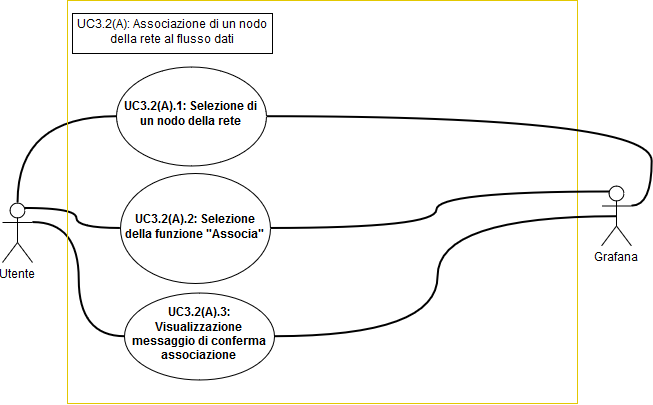
\includegraphics[width=\textwidth]{UC3-2(A).png}
                    	\caption{UC3.2(A): Associazione di un nodo della rete al flusso dati}
                    	\label{uc3.2a}
                    \end{figure}
                    
                \subsubsection{UC3.2(A).1: Selezione di un nodo della rete}
                    \textbf{Descrizione:} L’utente sceglie, tra quelli proposti, un nodo della rete che modellerà l'andamento del flusso dati.
                    \newline
                    \textbf{Precondizione:} E' stata selezionata una rete bayesiana all'interno della quale ricercare un nodo da associare al flusso dati precedentemente associato.
                    \newline
                    \textbf{Postcondizione:} E' stato scelto il nodo a cui associare il flusso di monitoraggio.
                    \newline
                    \textbf{Attore primario:} Utente.
                    \newline
                    \textbf{Attore secondario:} Grafana.
                    \newline
                    \textbf{Contestualizzazione / Scenario principale:} \begin{enumerate}
                        \item L’utente seleziona il nodo appartenente alla rete precedentemente selezionata che vuole associare da un elenco.
                    \end{enumerate}
                    
                \subsubsection{UC3.2(A).2: Selezione della funzione "Associa"}
                    \textbf{Descrizione:} L’utente associa il nodo precedentemente scelto al flusso dati.
                    \newline
                    \textbf{Precondizione:}  È stato selezionato il nodo a cui associare il flusso di monitoraggio.
                    \newline
                    \textbf{Postcondizione:} Il flusso dati è associato al nodo delle rete desiderato.
                    \newline
                    \textbf{Attore primario:} Utente.
                    \newline
                    \textbf{Attore secondario:} Grafana.
                    \newline
                    \textbf{Contestualizzazione / Scenario principale:} \begin{enumerate}
                        \item L’utente clicca sul pulsante "Associa" che attiva la funzione di associazione.
                    \end{enumerate} 
                
	           
	            \subsubsection{UC3.2(A).3: Visualizzazione messaggio di conferma associazione}
	                \textbf{Descrizione:} L’utente è a conoscenza che l'associazione è andata a buon fine.
	                \newline
                    \textbf{Precondizione:} Il nodo della rete bayesiana è stato associato al flusso di monitoraggio con successo.
                    \newline
                    \textbf{Postcondizione:} Il sistema mostra all'utente la conferma dell'associazione.
                    \newline
                    \textbf{Attore primario:} Utente.
                    \newline
                    \textbf{Attore secondario:} Grafana.
                    \newline
                    \textbf{Contestualizzazione / Scenario principale:} \begin{enumerate}
                        \item L'utente visualizza il messaggio di conferma associazione ("Associazione riuscita").
                    \end{enumerate}
                    
                
                    
                \subsubsection{UC3.2(B): Dissociazione del nodo della rete dal flusso dati}
                    \textbf{Descrizione:} L’utente vuole eliminare l'associazione precedente tra il flusso e il nodo della rete selezionata (Fig.\ref{uc3.2b}).
                    \newline
                    \textbf{Precondizione:} E' presente un'associazione di un nodo di quella rete con il flusso dati.
                    \newline
                    \textbf{Postcondizione:} E' stata rimossa l'associazione del nodo precedentemente associato al flusso dati.
                    \newline
                    \textbf{Attore primario:} Utente.
                    \newline
                    \textbf{Attore secondario:} Grafana.
                    \newline
                    \textbf{Contestualizzazione / Scenario principale:} 
                    \begin{enumerate}
                        \item Seleziona la funzione “Dissocia” \underline{\textit{UC3.2(B).1}};
                        \item Viene visualizzato un messaggio di conferma dissociazione (“Dissociazione riuscita”) \underline{\textit{UC3.2(B).2}}.   
                    \end{enumerate}    
                
                \begin{figure}[!htbp]
                	\centering
                	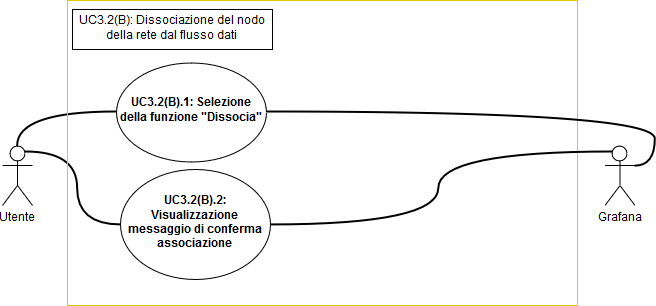
\includegraphics[width=\textwidth]{UC3-2(B).png}
                	\caption{UC3.2(B): Dissociazione del nodo della rete dal flusso dati}
                	\label{uc3.2b}
                \end{figure}
                
                \subsubsection{UC3.2(B).1: Selezione della funzione "Dissocia"}
                    \textbf{Descrizione:} L’utente seleziona la funzione dissocia.
                    \newline
                    \textbf{Precondizione:}  E' già presente un'associazione nodo-flusso dati per la rete selezionata.
                    \newline
                    \textbf{Postcondizione:} Il flusso dati non è più associato al nodo delle rete.
                    \newline
                    \textbf{Attore primario:} Utente.
                    \newline
                    \textbf{Attore secondario:} Grafana.
                    \newline
                    \textbf{Contestualizzazione / Scenario principale:} \begin{enumerate}
                        \item L’utente clicca sul pulsante "Dissocia" che attiva la funzione di dissociazione.
                    \end{enumerate} 
	           
	                
	            \subsubsection{UC3.2(B).2: Visualizzazione messaggio di conferma associazione}
	                \textbf{Descrizione:} L’utente è a conoscenza che la dissociazione è andata a buon fine.
	                \newline
                    \textbf{Precondizione:} Il nodo della rete bayesiana è stato dissociato dal flusso di monitoraggio con successo.
                    \newline
                    \textbf{Postcondizione:} Il sistema mostra all'utente la conferma della dissociazione.
                    \newline
                    \textbf{Attore primario:} Utente.
                    \newline
                    \textbf{Attore secondario:} Grafana.
                    \newline
                    \textbf{Contestualizzazione / Scenario principale:} \begin{enumerate}
                        \item L'utente visualizza il messaggio di conferma dissociazione ("Dissociazione riuscita").
                    \end{enumerate}
                    
                    
                    
                \subsubsection{UC4: Salvataggio Dashboard}
                    \textbf{Descrizione:} L’utente vuole salvare le modifiche della Dashboard corrente (Fig.\ref{uc4}).
                    \newline
                    \textbf{Precondizione:} L'utente deve trovarsi su una schermata di una dashboard.
                    \newline
                    \textbf{Postcondizione:} Avviene il salvataggio delle modifiche.
                    \newline
                    \textbf{Attore primario:} Utente.
                    \newline
                    \textbf{Attore secondario:} Grafana.
                    \newline
                    \textbf{Contestualizzazione / Scenario principale:} \begin{enumerate}
                        \item L'utente lancia la funzione di salvataggio Dashboard \underline{\textit{UC4.1}};
                        \item L'utente inserisce opzionalmente le note dei cambiamenti effettuati \underline{\textit{UC4.2}};
                        \item L'utente preme su "Save".
                    \end{enumerate}
                    \textbf{Estensioni:} \begin{enumerate}
                            \item C’è stato un problema con il salvataggio della Dashboard \underline{\textit{UC16}}.
                            \item L'utente decide di non voler salvare e preme su "Cancel" \underline{\textit{UC15}}.
                        \end{enumerate}
                \clearpage
                \begin{figure}[!htbp]
                    	\centering
                    	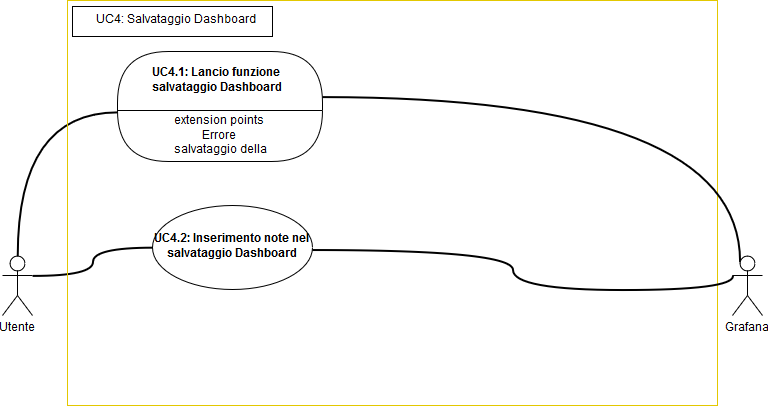
\includegraphics[width=\textwidth]{UC4.png}
                    	\caption{UC4 - Salvataggio Dashboard}
                    	\label{uc4}
                    \end{figure}   
                
                \subsubsection{UC4.1: Lancio funzione salvataggio Dashboard}
                    \textbf{Descrizione:} L’utente avvia la funzione di salvataggio di una Dashboard tramite comandi da tastiera o con l'apposito pulsante.
                    \newline
                    \textbf{Precondizione:} L'utente deve trovarsi su una schermata di una dashboard.
                    \newline
                    \textbf{Postcondizione:} Avviene il lancio della funzione di salvataggio della dashboard.
                    \newline
                    \textbf{Attore primario:} Utente.
                    \newline
                    \textbf{Attore secondario:} Grafana.
                    \newline
                    \textbf{Contestualizzazione / Scenario principale:} \begin{enumerate}
                        \item L'utente lancia la funzione di salvataggio Dashboard premendo sul pulsante apposito in alto a destra.
                    \end{enumerate}
                
                \subsubsection{UC4.1(A): Lancio funzione salvataggio Dashboard tramite pulsante}
                    \textbf{Descrizione:} L’utente preme sul pulsante apposito per il lancio della funzione di salvataggio.
                    \newline
                    \textbf{Precondizione:} L'utente deve trovarsi su una schermata di una dashboard.
                    \newline
                    \textbf{Postcondizione:} Avviene il lancio della funzione di salvataggio della dashboard.
                    \newline
                    \textbf{Attore primario:} Utente.
                    \newline
                    \textbf{Attore secondario:} Grafana.
                    \newline
                    \textbf{Contestualizzazione / Scenario principale:} \begin{enumerate}
                        \item L'utente lancia la funzione di salvataggio Dashboard premendo sul pulsante apposito in alto a destra.
                    \end{enumerate}
                
                \subsubsection{UC4.1(B): Lancio funzione salvataggio Dashboard tramite shortcut}
                    \textbf{Descrizione:} L’utente esegue il comando "CTRL+S" per il lancio della funzione di salvataggio.
                    \newline
                    \textbf{Precondizione:} L'utente deve trovarsi su una schermata di una dashboard.
                    \newline
                    \textbf{Postcondizione:} Avviene il lancio della funzione di salvataggio della dashboard.
                    \newline
                    \textbf{Attore primario:} Utente.
                    \newline
                    \textbf{Attore secondario:} Grafana.
                    \newline
                    \textbf{Contestualizzazione / Scenario principale:} \begin{enumerate}
                        \item L'utente lancia la funzione di salvataggio Dashboard tramite il comando "CTRL+S".
                    \end{enumerate}
                
                \subsubsection{UC4.2: Inserimento note nel salvataggio Dashboard}
                    \textbf{Descrizione:} L’utente vuole inserire delle note per identificare meglio i cambiamenti effettuati fino a questo salvataggio della Dashboard.
                    \newline
                    \textbf{Precondizione:} L'utente ha lanciato il salvataggio di una Dashboard.
                    \newline
                    \textbf{Postcondizione:} L'utente ha inserito le informazioni che ritiene più pertinenti.
                    \newline
                    \textbf{Attore primario:} Utente.
                    \newline
                    \textbf{Attore secondario:} Grafana.
                    \newline
                    \textbf{Contestualizzazione / Scenario principale:} \begin{enumerate}
                        \item L'utente inserisce le informazioni che ritiene importanti da mettere come note al salvataggio delle modifiche della Dashboard.
                    \end{enumerate}
                
                   
                          
                \subsubsection{UC5: Definizione di un alert personalizzato per un flusso dati non monitorato}
                    \textbf{Descrizione:} L’utente desidera creare un alert associato ad un flusso dati non monitorato su Grafana ed nella schermata di modifica di un panel (Fig.\ref{uc5}).
                    \newline
                    \textbf{Precondizione:} Sono presenti dei flussi dati non monitorati su Grafana.
                    \newline
                    \textbf{Postcondizione:} È stato definito un alert personalizzato per il flusso dati.
                    \newline
                    \textbf{Attore primario:} Utente.
                    \newline
                    \textbf{Attore secondario:} Grafana.
                    \newline
                    \textbf{Contestualizzazione / Scenario principale:} \begin{enumerate}
                            \item L'utente preme sul panel "Alert" \underline{\textit{UC6}};
                            \item L’utente preme sul pulsante “Create alert” \underline{\textit{UC5.1}};
                            \item L'utente modifica i dati dell'alert\underline{\textit{UC7}};
                            \item L'utente definisce la notifica dell'alert \underline{\textit{UC5.2}}.
                        \end{enumerate}
                        
                        
                        \begin{figure}[!htbp]
                    	\centering
                    	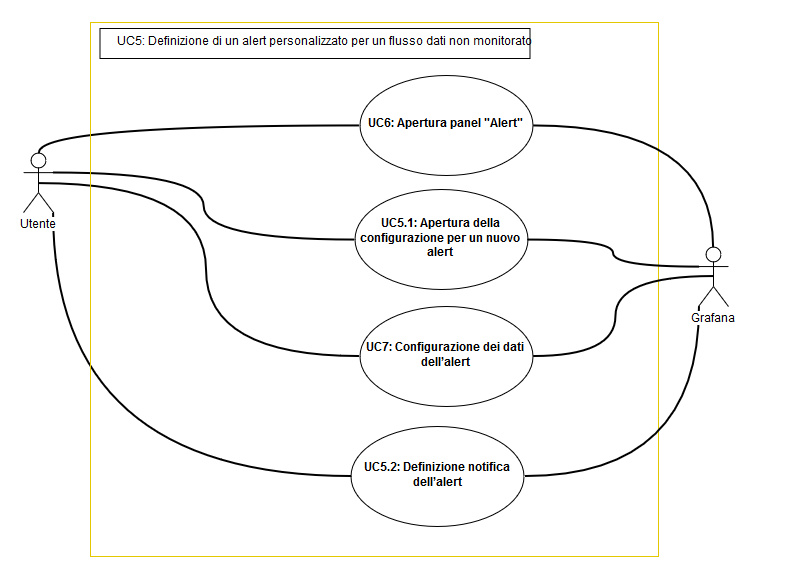
\includegraphics[width=\textwidth]{UC5.png}
                    	\caption{UC5 - Definizione di un alert personalizzato per un flusso dati non monitorato}
                    	\label{uc5}
                    \end{figure} 
                    \clearpage
                \subsubsection{UC5.1: Apertura della configurazione per un nuovo alert}
                    \textbf{Descrizione:} L’utente preme sul pulsante "Create Alert" per creare un nuovo alert.
                    \newline
                    \textbf{Precondizione:} L'utente visualizza il panel "alert".
                    \newline
                    \textbf{Postcondizione:} Sono disponibili i campi precompilati per la creazione di un alert.
                    \newline
                    \textbf{Attore primario:} Utente.
                    \newline
                    \textbf{Attore secondario:} Grafana.
                    \newline
                    \textbf{Contestualizzazione / Scenario principale:} \begin{enumerate}
                            \item L’utente preme sul pulsante "Create Alert".
                        \end{enumerate}  
                        
                        
                        
                    
                \subsubsection{UC5.2: Definizione notifica dell'alert }
                    \textbf{Descrizione:} L’utente preme sul pulsante "Notifications" per definire come ricevere e cosa scrivere nella notifica che invierà l'alert (Fig.\ref{uc5.2}).
                    \newline
                    \textbf{Precondizione:} L'utente si trova nel panel "Alert".
                    \newline
                    \textbf{Postcondizione:} Destinatario e descrizione dell'alert sono definiti.
                    \newline
                    \textbf{Attore primario:} Utente.
                    \newline
                    \textbf{Attore secondario:} Grafana.
                    \newline
                    \textbf{Contestualizzazione / Scenario principale:} \begin{enumerate}
                            \item L'utente preme sul pulsante "Notifications";
                            \item L'utente aggiunge un destinatario \underline{\textit{UC5.2.1}};
                            \item L'utente scrive un messaggio \underline{\textit{UC5.2.2}}.
                        \end{enumerate}
                        \clearpage
                        \begin{figure}[!htbp]
                    	\centering
                    	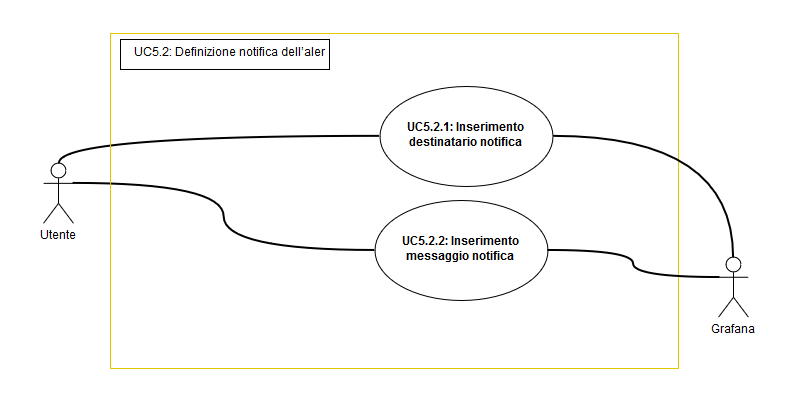
\includegraphics[width=\textwidth]{UC5-2.png}
                    	\caption{UC5.2 - Definizione notifica dell'alert}
                    	\label{uc5.2}
                    \end{figure}  
                        
                \subsubsection{UC5.2.1: Inserimento destinatario notifica }
                    \textbf{Descrizione:} L’utente inserisce nel form "Send to" il destinatario della notifica.
                    \newline
                    \textbf{Precondizione:} L'utente é nella sezione "Notifications" .
                    \newline
                    \textbf{Postcondizione:} Il contatto per il destinatario é inserito.
                    \newline
                    \textbf{Attore primario:} Utente.
                    \newline
                    \textbf{Attore secondario:} Grafana.
                    \newline
                    \textbf{Contestualizzazione / Scenario principale:} \begin{enumerate}
                            \item L'utente inserisce il destinatario della notifica.
                        \end{enumerate}        
                
                
                \subsubsection{UC5.2.2: Inserimento messaggio notifica }
                    \textbf{Descrizione:} L’utente inserisce nel form "Message" il messaggio della notifica.
                    \newline
                    \textbf{Precondizione:} L'utente é nella sezione "Notifications" .
                    \newline
                    \textbf{Postcondizione:} Il messaggio della notifica é inserito.
                    \newline
                    \textbf{Attore primario:} Utente.
                    \newline
                    \textbf{Attore secondario:} Grafana.
                    \newline
                    \textbf{Contestualizzazione / Scenario principale:} \begin{enumerate}
                            \item L'utente inserisce il messaggio della notifica.
                        \end{enumerate} 
                 
                \subsubsection{UC6: Apertura panel "Alert"}
                    \textbf{Descrizione:} L’utente preme sul panel per visualizzare l'alert.
                    \newline
                    \textbf{Precondizione:} L'utente si trova nella dashboard del plugin.
                    \newline
                    \textbf{Postcondizione:} Il panel per visualizzare un alert é aperto.
                    \newline
                    \textbf{Attore primario:} Utente.
                    \newline
                    \textbf{Attore secondario:} Grafana.
                    \newline
                    \textbf{Contestualizzazione / Scenario principale:} \begin{enumerate}
                            \item L’utente preme sul panel "Alert".
                        \end{enumerate}   
                    
                        
                        
                     		
                \subsubsection{UC7: Configurazione dei dati dell'alert}
                    \textbf{Descrizione:} L’utente modifica i campi precompilati per la configurazione di un alert (Fig.\ref{uc7}).
                    \newline
                    \textbf{Precondizione:} L'utente si trova nel panel alert.
                    \newline
                    \textbf{Postcondizione:} L'alert é configurato.
                    \newline
                    \textbf{Attore primario:} Utente.
                    \newline
                    \textbf{Attore secondario:} Grafana.
                    \newline
                    \textbf{Contestualizzazione / Scenario principale:} \begin{enumerate}
                            \item L’utente modifica il nome dell'alert \underline{\textit{UC7.1}};
                            \item L'utente modifica il valore "Evaluate every" \underline{\textit{UC7.2}};
                            \item L'utente modifica il valore "For" \underline{\textit{UC7.3}};
                            \item L'utente può aggiungere una condizione \underline{\textit{UC7.4}};
                            \item L'utente modifica una condizione \underline{\textit{UC7.5}};
                            \item L'utente può cancellare una condizione \underline{\textit{UC7.6}};
                            \item L'utente sceglie lo stato nel caso non ci siano valori o tutti i valori siano nulli \underline{\textit{UC7.7}};
                            \item L'utente testa le condizioni \underline{\textit{UC7.8}}.
                        \end{enumerate}
                        
                \textbf{Estensioni:} 
                    \begin{enumerate}
                            \item Errore nei dati inseriti per la configurazione dell'alert \underline{\textit{UC13}}.
                        \end{enumerate}
        
        \begin{figure}[!htbp]
                    	\centering
                    	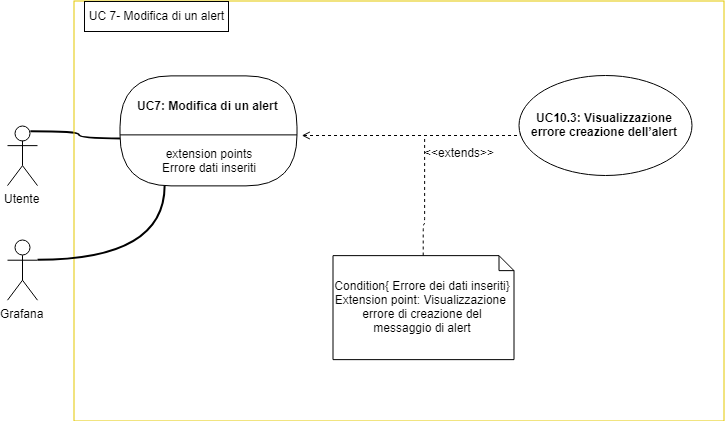
\includegraphics[width=\textwidth]{UC7.png}
                    	\caption{UC7 - Configurazione dei dati dell'alert}
                    	\label{uc7}
                    \end{figure} 
                
                \subsubsection{UC7.1: Modifica nome dell'alert}
                    \textbf{Descrizione:} L’utente modifica il nome dell'alert nell'apposito form.
                    \newline
                    \textbf{Precondizione:} Il sistema visualizza il form per la scrittura del nome dell'alert.
                    \newline
                    \textbf{Postcondizione:} Il nuovo nome dell'alert é inserito.
                    \newline
                    \textbf{Attore primario:} Utente.
                    \newline
                    \textbf{Attore secondario:} Grafana.
                    \newline
                    \textbf{Contestualizzazione / Scenario principale:} \begin{enumerate}
                            \item L’utente modifica il nome dell'alert.
                        \end{enumerate}
                        
                \subsubsection{UC7.2: Modifica tempo di valutazione condizione alert}
                    \textbf{Descrizione:} L’utente modifica il valore per definire ogni quanto tempo Grafana controllerà la validità delle condizioni dell'alert.  
                    \newline
                    \textbf{Precondizione:} Il sistema visualizza il form "Evaluate every" per la scrittura del valore.
                    \newline
                    \textbf{Postcondizione:} Il valore "Evaluate every" é modificato.
                    \newline
                    \textbf{Attore primario:} Utente.
                    \newline
                    \textbf{Attore secondario:} Grafana.
                    \newline
                    \textbf{Contestualizzazione / Scenario principale:} \begin{enumerate}
                            \item L'utente modifica il valore "Evaluate every".
                        \end{enumerate}
                
                \subsubsection{UC7.3: Modifica soglia di tolleranza per lancio di un alert}
                    \textbf{Descrizione:} L’utente modifica il valore per definire la tolleranza temporale prima del lancio di un alert.  
                    \newline
                    \textbf{Precondizione:} Il sistema visualizza il form "For" per la scrittura del valore.
                    \newline
                    \textbf{Postcondizione:} Il valore "For" é modificato.
                    \newline
                    \textbf{Attore primario:} Utente.
                    \newline
                    \textbf{Attore secondario:} Grafana.
                    \newline
                    \textbf{Contestualizzazione / Scenario principale:} \begin{enumerate}
                            \item L'utente modifica il valore "For" .
                        \end{enumerate}
                
                
                \subsubsection{UC7.4: Aggiunta condizione }
                    \textbf{Descrizione:} L’utente può aggiungere una condizione sotto forma di query premendo sul pulsante "+".
                    \newline
                    \textbf{Precondizione:} Il sistema visualizza il form "Conditions" per la definizione della condizione.
                    \newline
                    \textbf{Postcondizione:} La condizione é pronta ad essere definita.
                    \newline
                    \textbf{Attore primario:} Utente.
                    \newline
                    \textbf{Attore secondario:} Grafana.
                    \newline
                    \textbf{Contestualizzazione / Scenario principale:} \begin{enumerate}
                            \item L'utente può aggiungere una condizione;
                        \end{enumerate}   
                      
                \subsubsection{UC7.5: Modifica condizione }
                    \textbf{Descrizione:} L’utente modifica la condizione su cui si baserà Grafana per il lancio dell'alert.
                    \newline
                    \textbf{Precondizione:} Il sistema visualizza il form "Conditions" e almeno una condizione deve essere presente.
                    \newline
                    \textbf{Postcondizione:} Una condizione é modificata.
                    \newline
                    \textbf{Attore primario:} Utente.
                    \newline
                    \textbf{Attore secondario:} Grafana.
                    \newline
                    \textbf{Contestualizzazione / Scenario principale:} \begin{enumerate}
                            \item L'utente modifica una condizione .
                        \end{enumerate}  
                
                
                
                \subsubsection{UC7.6: Eliminazione condizione }
                    \textbf{Descrizione:} L’utente può eliminare una condizione premendo sul pulsante con simbolo un cestino.
                    \newline
                    \textbf{Precondizione:} Il sistema visualizza il form "Conditions" e deve essere presente almeno una condizione.
                    \newline
                    \textbf{Postcondizione:} Una condizione é eliminata.
                    \newline
                    \textbf{Attore primario:} Utente.
                    \newline
                    \textbf{Attore secondario:} Grafana.
                    \newline
                    \textbf{Contestualizzazione / Scenario principale:} \begin{enumerate}
                            \item L'utente può eliminare una condizione.
                        \end{enumerate}
                        
                \subsubsection{UC7.7: Modifica dello stato del sistema nel caso non ci siano valori o tutti i valori siano nulli }
                    \textbf{Descrizione:} L’utente modifica lo stato in cui sarà il sistema nel caso non ci siano dati o tutti i valori siano nulli.
                    \newline
                    \textbf{Precondizione:} Il sistema visualizza il form "If no data or all values are null".
                    \newline
                    \textbf{Postcondizione:} Lo stato é definito.
                    \newline
                    \textbf{Attore primario:} Utente.
                    \newline
                    \textbf{Attore secondario:} Grafana.
                    \newline
                    \textbf{Contestualizzazione / Scenario principale:} \begin{enumerate}
                            \item L'utente modifica lo stato del sistema nel caso non ci siano valori o tutti i valori siano nulli.
                        \end{enumerate}
                        
                 \subsubsection{UC7.8: Test delle condizioni }
                    \textbf{Descrizione:} L’utente preme sul pulsante "Test Rule" per testare se le condizioni.
                    \newline
                    \textbf{Precondizione:} Tutti i form per definire un alert sono compilati .
                    \newline
                    \textbf{Postcondizione:} L'utente visualizza i risultati del test.
                    \newline
                    \textbf{Attore primario:} Utente.
                    \newline
                    \textbf{Attore secondario:} Grafana.
                    \newline
                    \textbf{Contestualizzazione / Scenario principale:} \begin{enumerate}
                            \item L'utente testa le condizioni.
                        \end{enumerate}
                        
                        
                		
            
                      		
               \subsubsection{UC8: Modifica di un alert}
                    \textbf{Descrizione:} L’utente desidera modificare un alert associato ad un flusso dati non monitorato su Grafana ed è già sulla sezione "alert" all'interno della sezione "modifica" di un panel (Fig.\ref{uc8}).
                    \newline
                    \textbf{Precondizione:} Sono presenti dei flussi dati non monitorati su Grafana e esiste un alert a loro associato.
                    \newline
                    \textbf{Postcondizione:} È stato modificato un alert personalizzato per il flusso dati.
                    \newline
                    \textbf{Attore primario:} Utente.
                    \newline
                    \textbf{Attore secondario:} Grafana.
                    \newline
                    \textbf{Contestualizzazione / Scenario principale:} \begin{enumerate}
                            \item L'utente preme sul panel "Alert" \underline{\textit{UC6}};
                            \item L'utente modifica i dati dell'alert \underline{\textit{UC7}};
                            \item L'utente modifica la notifica dell'alert \underline{\textit{UC8.1}}.
                        \end{enumerate}
                    
                    \textbf{Estensioni:} 
                    \begin{enumerate}
                            \item Errore nei dati inseriti per la creazione dell'alert \underline{\textit{UC13}}.
                        \end{enumerate} 		
                		
                        \begin{figure}[!htbp]
                    	\centering
                    	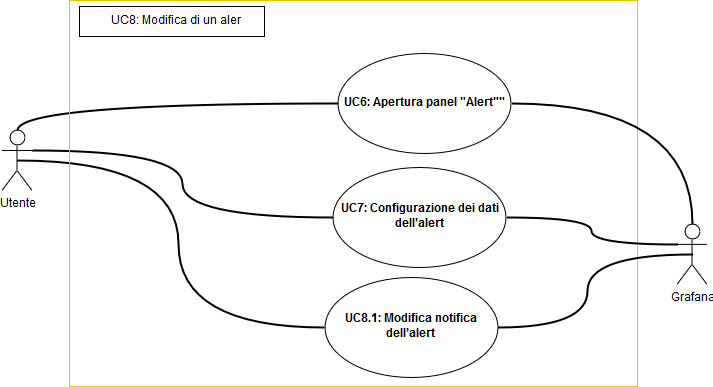
\includegraphics[width=\textwidth]{UC8.png}
                    	\caption{UC8 - Modifica di un alert}
                    	\label{uc8}
                    \end{figure}
                        
                      
                \subsubsection{UC8.1: Modifica notifica dell'alert }
                    \textbf{Descrizione:} L’utente preme sul pulsante "Notifications" per modificare il metodo di ricevimento e il contenuto della notifica (Fig.\ref{uc8.1}).
                    \newline
                    \textbf{Precondizione:} L'utente si trova nel panel "Alert".
                    \newline
                    \textbf{Postcondizione:} Destinatario e descrizione dell'alert sono modificati.
                    \newline
                    \textbf{Attore primario:} Utente.
                    \newline
                    \textbf{Attore secondario:} Grafana.
                    \newline
                    \textbf{Contestualizzazione / Scenario principale:} \begin{enumerate}
                            \item L'utente preme sul pulsante "Notifications";
                            \item L'utente modifica il destinatario \underline{\textit{UC8.1.1}};
                            \item L'utente modifica il messaggio \underline{\textit{UC8.1.2}}.
                        \end{enumerate}
                        
                         \begin{figure}[!htbp]
                    	\centering
                    	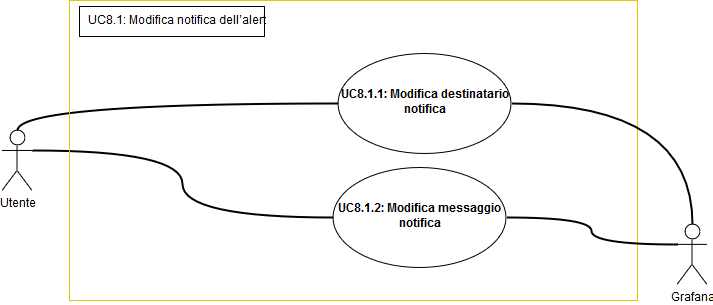
\includegraphics[width=\textwidth]{UC8-1.png}
                    	\caption{UC8.1 - Modifica notifica dell'alert}
                    	\label{uc8.1}
                    \end{figure}
                        
                \subsubsection{UC8.1.1: Modifica destinatario notifica }
                    \textbf{Descrizione:} L’utente modifica nel form "Send to" il destinatario della notifica.
                    \newline
                    \textbf{Precondizione:} L'utente é nella sezione "Notifications" .
                    \newline
                    \textbf{Postcondizione:} Il contatto per il destinatario é modificato.
                    \newline
                    \textbf{Attore primario:} Utente.
                    \newline
                    \textbf{Attore secondario:} Grafana.
                    \newline
                    \textbf{Contestualizzazione / Scenario principale:} \begin{enumerate}
                            \item L'utente modifica il destinatario della notifica.
                        \end{enumerate}        
                
                
                \subsubsection{UC8.1.2: Modifica messaggio notifica }
                    \textbf{Descrizione:} L’utente modifica nel form "Message" il messaggio della notifica.
                    \newline
                    \textbf{Precondizione:} L'utente é nella sezione "Notifications" .
                    \newline
                    \textbf{Postcondizione:} Il messaggio della notifica é modificato.
                    \newline
                    \textbf{Attore primario:} Utente.
                    \newline
                    \textbf{Attore secondario:} Grafana.
                    \newline
                    \textbf{Contestualizzazione / Scenario principale:} \begin{enumerate}
                            \item L'utente modifica il messaggio della notifica.
                        \end{enumerate} 		
                		
                		
                		
                    
                \subsubsection{UC9: Rimozione di un alert}
                    \textbf{Descrizione:}  L’utente desidera eliminare un alert associato ad un flusso dati non monitorato su Grafana (Fig.\ref{uc9}).
                    \newline
                    \textbf{Precondizione:} Sono presenti dei flussi dati non monitorati su Grafana ed esiste un alert a loro associato.
                    \newline
                    \textbf{Postcondizione:} Non é presente un alert personalizzato per il flusso dati.
                    \newline
                    \textbf{Attore primario:} Utente.
                    \newline
                    \textbf{Attore secondario:} Grafana.
                    \newline
                    \textbf{Contestualizzazione / Scenario principale:} \begin{enumerate}
                            \item L'utente preme sul panel "Alert" \underline{\textit{UC6}};
                            \item L’utente preme sul pulsante “Delete”;
                            \item L’utente visualizza un messaggio di richiesta di conferma di cancellazione \underline{\textit{UC9.1}}.
                        \end{enumerate}
                    
                    \textbf{Estensioni:} 
                    \begin{enumerate}
                            \item L'utente preme sul pulsante "Cancel" nel momento di conferma cancellazione. \underline{\textit{UC17}}.
                        \end{enumerate}
                        
                        \begin{figure}[!htbp]
                    	\centering
                    	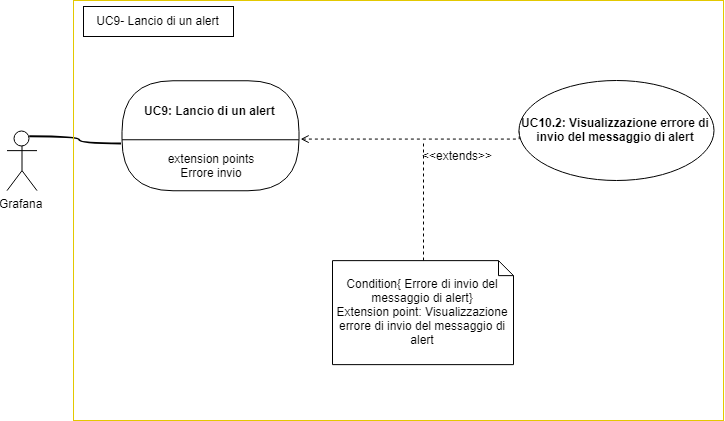
\includegraphics[width=\textwidth]{UC9.png}
                    	\caption{UC9 - Rimozione di un alert}
                    	\label{uc9}
                    \end{figure}   
                        
                \subsubsection{UC9.1: Visualizzazione messaggio di conferma cancellazione alert}
                    \textbf{Descrizione:}  L’utente può confermare l'operazione di cancellazione dell'alert oppure annullarla.
                    \newline
                    \textbf{Precondizione:} L'utente ha premuto su "Delete".
                    \newline
                    \textbf{Postcondizione:} Non é presente un alert personalizzato per il flusso dati.
                    \newline
                    \textbf{Attore primario:} Utente.
                    \newline
                    \textbf{Attore secondario:} Grafana.
                    \newline
                    \textbf{Contestualizzazione / Scenario principale:} \begin{enumerate}
                            \item L'utente visualizza un messaggio di richiesta di conferma di cancellazione.
                            \item L'utente preme su "Delete".
                        \end{enumerate}
                \textbf{Estensioni:} 
                    \begin{enumerate}
                            \item L'utente preme sul pulsante "Cancel" nel momento di conferma cancellazione. \underline{\textit{UC17}}.
                        \end{enumerate}
				
		\subsection{Attore primario: Grafana}	
		
		        \subsubsection{UC10: Lancio di un alert}
                    \textbf{Descrizione:} Grafana ha rilevato che una delle condizioni dell'alert sono state violate e avviene quindi il "lancio" dell'alert stesso.
                    \newline
                    \textbf{Precondizione:} Il flusso di monitoraggio\pedice di interesse ha un alert ed è associato ad un nodo di una rete bayesiana, inoltre, il valore corrente del flusso è entro il range di valori impostati nelle condizioni dell'alert associato.
                    \newline
                    \textbf{Postcondizione:} Vengono interpretati i dati per il ricalcolo delle probabilità con il contributo di “jsbayes”.
                    \newline
                    \textbf{Attore primario:} Grafana.
                    \newline
                    \textbf{Contestualizzazione / Scenario principale:} \begin{enumerate}
                            \item Grafana rileva che un flusso di monitoraggio\pedice rispetta le condizioni di uno dei suoi alert;
                            \item Si apre una finestra per visualizzare i dati riguardanti il nodo associato al flusso di monitoraggio e la condizione che ha fatto scattare l'alert;
                            \item La libreria jsbayes ricalcola le probabilità dei nodi non monitorati.
                        \end{enumerate}
                    
                    \textbf{Estensioni:} 
                    \begin{enumerate}
                        \item Viene visualizzato un errore di invio messaggio di alert. \underline{\textit{UC12}}.
                    \end{enumerate}
                    
                      
                      
                \subsubsection{UC11: Visualizzazione errore interpretazione rete Bayesiana}
                    \textbf{Descrizione:} Il sistema avvisa l’utente che la rete Bayesiana non è stata interpretata correttamente e non può essere inserita (Fig.\ref{uc11}).
                    \newline
                    \textbf{Precondizione:} L’utente inserisce una rete Bayesiana non formattata correttamente.
                    \newline
                    \textbf{Postcondizione:} L’utente è consapevole di aver inserito una rete Bayesiana non formattata correttamente.
                    \newline
                    \textbf{Attore primario:} Grafana.
                    \newline
                    \textbf{Attore secondario:} Utente.
                    \newline
                    \textbf{Contestualizzazione / Scenario principale:} \begin{enumerate}
                            \item il sistema avvisa l'utente aprendo una finestra che mostra un messaggio di errore;
                            \item L'utente chiude il messaggio di avviso premendo su "Ok", \underline{\textit{UC14}};
                            \item L'utente viene rimandato all'interfaccia di upload in modo che abbia la possibilità di inserire una nuova rete, \underline{\textit{UC1}};.
                        \end{enumerate}
                
                \begin{figure}[!htbp]
                    	\centering
                    	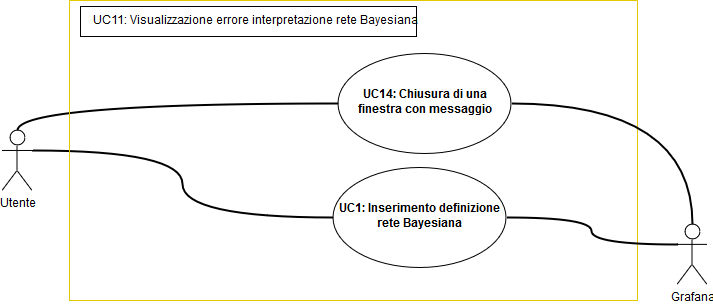
\includegraphics[width=\textwidth]{UC11.png}
                    	\caption{UC11 - Visualizzazione errore interpretazione rete Bayesiana}
                    	\label{uc11}
                    \end{figure}
                
                \subsubsection{UC12: Visualizzazione errore invio del messaggio di alert}
                    \textbf{Descrizione:} Il sistema avvisa l'utente che e’ avvenuto un errore nell'invio dell'alert.
                    \newline
                    \textbf{Precondizione:} E’ avvenuto un errore nell'invio dell'alert da parte di Grafana.
                    \newline
                    \textbf{Postcondizione:} L’utente è consapevole dell'errore nell'invio dell'alert.
                    \newline
                    \textbf{Attore primario:} Grafana.
                    \newline
                    \textbf{Attore secondario:} Utente.
                    \newline
                    \textbf{Contestualizzazione / Scenario principale:} \begin{enumerate}
                            \item Il sistema apre una finestra con il messaggio di fallimento dell'alert;
                            \item l'utente chiude il messaggio di avviso premendo su "Ok" \underline{\textit{UC14}};.
                        \end{enumerate}
                        
                \subsubsection{UC13: Visualizzazione errore configurazione dell'alert}
                    \textbf{Descrizione:} Il sistema avvisa l’utente che è avvenuto un errore nella configurazione dell'alert.
                    \newline
                    \textbf{Precondizione:} E' avvenuto un errore nell'inserimento dei dati nell'alert da parte dell'utente.
                    \newline
                    \textbf{Postcondizione:} L’utente è consapevole dell'errore nella creazione dell'alert.
                    \newline
                    \textbf{Attore primario:} Grafana.
                    \newline
                    \textbf{Attore secondario:} Utente.
                    \newline
                    \textbf{Contestualizzazione / Scenario principale:} \begin{enumerate}
                            \item Il sistema avvisa l’utente tramite un messaggio di errore;
                            \item L'utente chiude il messaggio di avviso premendo su "Ok" \underline{\textit{UC14}}.
                        \end{enumerate}
                        
                \subsubsection{UC14: Chiusura di una finestra con messaggio}
                    \textbf{Descrizione:} L'utente visualizza un messaggio e poi chiude la finestra che lo contiene.
                    \newline
                    \textbf{Precondizione:} E' aperta una finestra con un messaggio da dare all'utente ed un pulsante "Ok" per chiuderla.
                    \newline
                    \textbf{Postcondizione:} L'utente ha chiuso la finestra.
                    \newline
                    \textbf{Attore primario:} Utente.
                    \newline
                    \textbf{Attore secondario:} Grafana.
                    \newline
                    \textbf{Contestualizzazione / Scenario principale:} \begin{enumerate}
                            \item L'utente chiude il messaggio di avviso premendo su "Ok".
                        \end{enumerate}
                        
                \subsubsection{UC15: Annullamento salvataggio dashboard}
                    \textbf{Descrizione:} Viene annullata l'operazione di salvataggio dei nuovi dati inseriti nella dashboard.
                    \newline
                    \textbf{Precondizione:} L'utente preme il pulsante "Cancel" nella finestra di salvataggio della dashboard. 
                    \newline
                    \textbf{Postcondizione:} Sono annullate le modifiche effettuate sulla dashboard.
                    \newline
                    \textbf{Attore primario:} Utente.
                    \newline
                    \textbf{Attore secondario:} Grafana.
                    \newline
                    \textbf{Contestualizzazione / Scenario principale:} \begin{enumerate}
                            \item L'utente torna alla schermata della dashboard perdendo le ultime modifiche effettuate.
                        \end{enumerate}
                        
                    \subsubsection{UC16: Errore salvataggio dashboard}
                    \textbf{Descrizione:} L'utente tenta di salvare le modifiche effettuate alla dashboard ma un errore ne impedisce il salvataggio.
                    \newline
                    \textbf{Precondizione:} L'utente preme il pulsante "Save" nell'apposita finestra per salvare le modifiche alla dashboard.
                    \newline
                    \textbf{Postcondizione:} L'utente viene rimandato alla dashboard perdendo le modifiche effettuate.
                    \newline
                    \textbf{Attore primario:} Utente.
                    \newline
                    \textbf{Attore secondario:} Grafana.
                    \newline
                    \textbf{Contestualizzazione / Scenario principale:} \begin{enumerate}
                            \item L'utente torna alla schermata della dashboard perdendo le ultime modifiche effettuate.
                        \end{enumerate}
                        
                    \subsubsection{UC17: Annullamento cancellazione alert}
                    \textbf{Descrizione:} Viene annullata l'operazione di cancellazione dell'alert.
                    \newline
                    \textbf{Precondizione:} L'utente non vuole cancellare l'alert.
                    \newline
                    \textbf{Postcondizione:} È annullata l'operazione di cancellazione dell'alert.
                    \newline
                    \textbf{Attore primario:} Utente.
                    \newline
                    \textbf{Attore secondario:} Grafana.
                    \newline
                    \textbf{Contestualizzazione / Scenario principale:} \begin{enumerate}
                            \item L'utente preme il pulsante "Cancel".
                            
                        \end{enumerate}
\newpage



	\section{Requisiti}
    Tracciare i requisiti significa che requisiti correlati vengono raggruppati e collegati per facilitare la lettura grazie a tabelle e indicizizzazioni.
    Assegneremo per tanto ad ogni requisito un identificatore univoco, composto da una serie di regole dettate dalla caratteristica stessa del requisiti.
    
    Verificabilità dei requisiti
    • I requisiti vanno scritti in modo che possano essere
    oggettivamente verificati nel prodotto finale
    • Occorre quantificare il tasso degli errori.
    – “Gli operatori esperti dovrebbero poter controllare le
    funzioni di sistema dopo due ore di formazione.
    Dopo tale formazione, il numero medio di errori
    degli operatori esperti non dovrebbe superare i due
    al giorno”
    
    Validazione dei requisiti
    • La dimostrazione che i requisiti definiscono il
    sistema davvero voluto dal cliente
    • La tecnica più importante di validazione dei
    requisiti è la prototipazione


    Analizzeremo nella seguente sezione i vari requisiti suddivisi in categorie:
    \begin{itemize}
        \item Funzionali
        \item Non funzionali:
            \begin{itemize}
                \item Requisiti di vincolo
                \item Requisiti di qualità
                \item Requisiti prestazionali
            \end{itemize}
    \end{itemize}
		\subsection{Requisiti Funzionali}			
        Descrivono in dettaglio i servizi che verranno forniti dal sistema agli attori.
        
        \subsection{Requisiti Non Funzionali}
        Descrivono i vincoli sul sistema e sul suo processo di sviluppo
        \subsubsection{Requisiti di vincolo}
        
        \subsubsection{Requisiti di qualità}
        \subsubsection{Requisiti prestazionali}

	
	\section{Tracciamento dei Requisiti}

\subsection{Tracciamento Casi d'Uso e Requisiti Funzionali}
Per una maggiore comprensione dei requisiti verranno rappresentate, in forma tabellare, le relazioni tra requisiti funzionali e casi d'uso. Il tracciamento diretto tra casi d'uso e requisiti renderà la comprensione del sistema più facile e veloce.
\clearpage

\begin{table}[!htbp] % h! serve per posizionarla relativamente
            \centering
            \renewcommand{\arraystretch}{2} % dimensione verticale delle righe
            \rowcolors{2}{gray!25}{white} %colori alternati, grigio 25% e bianco 100%
            \begin{tabular}{|c|c|} % p{dimensione desiderata}
                \rowcolor{orange!50} %colore intestazione
        		\hline
        		\textbf{Codice Caso d'Uso} & \textbf{Codice Requisito} \\
                \hline
                UC1 & RFC1\\
                \hline
                UC1(A) & RFC1A\\
                \hline
                UC1(A).1 & RFC1A.1\\
                \hline
                UC1(B) & RFC1B\\
                \hline
                UC2 & RFC2\\
                \hline
                UC2.1 & RFCC2.1\\
                \hline
                UC2.2 & RFC2.2\\
                \hline
                UC2.3 & RFC2.3\\
                \hline
                UC2.3.1 & RFC2.3.1\\
                \hline
                UC2.3.2 & RFC2.3.2\\
                \hline
                UC3 & RFC3\\
                \hline
                UC3.1 & RFC3.1\\
                \hline
                UC3.2 & RFC3.2\\
                \hline
                UC3.2(A)& RFC3.2A\\
                \hline
                UC3.2(A).1 & RFC3.2A.1\\
                \hline
                UC3.2(A).2 & RFC3.2A.2\\
                \hline
                UC3.2(A).3 & RFC3.2.3\\
                \hline
                \end{tabular}
        \end{table}

        \begin{table}[!htbp] % h! serve per posizionarla relativamente
            \centering
            \renewcommand{\arraystretch}{2} % dimensione verticale delle righe
            \rowcolors{2}{gray!25}{white} %colori alternati, grigio 25% e bianco 100%
                \begin{tabular}{|c|c|} % p{dimensione desiderata}
                \rowcolor{orange!50} %colore intestazione
        		\hline
        		\textbf{Codice Caso d'Uso} & \textbf{Codice Requisito} \\
                \hline
                UC3.2(B) & RFC3.2B\\
                \hline
                UC3.2(B).1 & RFC3.2B.1\\
                \hline
                UC3.2(B).2 & RFC3.2B.2\\
                \hline
                UC4 & RFC4\\
                \hline
                UC4.1 & RFC4.1\\
                \hline
                UC4.1(A) & RFC4.1A\\
                \hline
                UC4.1(B) & RFC4.1B\\
                \hline
                UC4.2 & RFC4.2\\
                \hline
                UC5 & RFO5\\
                \hline
                UC5.1 & RFO5.1\\
                \hline
                UC5.2 & RFO5.2\\
                \hline
                UC5.2.1 & RFO5.2.1\\
                \hline
                UC5.2.2 & RFO5.2.2\\
                \hline
                UC6 & RFC6\\
                \hline
                UC7 & RFC7\\
                \hline
                UC7.1 & RFC7.1\\
                \hline
                UC7.2 & RFC7.2\\
                \hline
                UC7.3 & RFC7.3\\
                \hline
                \end{tabular}
        \end{table}

        \begin{table}[!htbp] % h! serve per posizionarla relativamente
            \centering
            \renewcommand{\arraystretch}{2} % dimensione verticale delle righe
            \rowcolors{2}{gray!25}{white} %colori alternati, grigio 25% e bianco 100%
                \begin{tabular}{|c|c|} % p{dimensione desiderata}
                \rowcolor{orange!50} %colore intestazione
                \hline
        		\textbf{Codice Caso d'Uso} & \textbf{Codice Requisito} \\
                \hline
                UC7.4 & RFC7.4\\
                \hline
                UC7.5 & RFC7.5\\
                \hline
                UC7.6 & RFC7.6\\
                \hline
                UC7.7 & RFC7.7\\
                \hline
                UC7.8 & RFC7.8\\
                \hline
                UC8 & RFC8\\
                \hline
                UC8.1 & RFC8.1\\
                \hline
                UC8.1.1 & RFC8.1.1\\
                \hline
                UC8.1.2 & RFC8.1.2\\
                \hline
                UC9 & RFC9\\
                \hline
                UC9.1 & RFC9.1\\
                \hline
                UC10 & RFC10\\
                \hline
                UC11 & RFC11\\
                \hline
                UC12 & RFC12\\
                \hline
                UC13 & RFC13\\
                \hline
                UC14 & RFC14\\
                \hline
                \end{tabular}
        \end{table}

        \begin{table}[!htbp] % h! serve per posizionarla relativamente
            \centering
            \renewcommand{\arraystretch}{2} % dimensione verticale delle righe
            \rowcolors{2}{gray!25}{white} %colori alternati, grigio 25% e bianco 100%
                \begin{tabular}{|c|c|} % p{dimensione desiderata}
                \rowcolor{orange!50} %colore intestazione
                \hline
        		\textbf{Codice Caso d'Uso} & \textbf{Codice Requisito} \\
        		\hline
                UC15 & RFC15\\
                \hline
                UC16 & RFC16\\
                \hline
                UC17 & RFC17\\
                \hline
        \end{tabular}
        \caption{Tracciamento Casi d'Uso - Requisiti Funzionali} %descrizone a fine tabella
\end{table}

\subsection{Tracciamento Requisiti per Tipologia e Priorità}
Per facilitare la lettura e la visualizzazione verranno presentate delle tabelle indicizzate in modo specifico:
\begin{itemize}
    \item Tracciamento Priorità-Requisito
    \item Tracciamento Tipologia-Requisito
\end{itemize}

\newpage
\subsubsection{Tracciamento: Priorità-Requisito}
Di seguito viene riportata una tabella riassuntiva che descrive le priorità dei requisiti e i requisiti che vi appartenengono per rendere di più facile lettura la distribuzione per priorità.
Per brevità non viene riportata la descrizione del requisito ma semplicemente il suo codice univoco in quando era già stato descritto in dettaglio nella sezioni precedenti.   

\begin{table}[!htbp] % h! serve per posizionarla relativamente
            \centering
            \renewcommand{\arraystretch}{2} % dimensione verticale delle righe
            \rowcolors{2}{gray!25}{white} %colori alternati, grigio 25% e bianco 100%
            \begin{tabular}{|c|p{2cm}|} % p{dimensione desiderata}
                \rowcolor{orange!50} %colore intestazione
        		\hline
        		\textbf{Priorità Requisito} & \textbf{Codice Requisiti} \\
                \hline
                Compulsory & RFC1, RFC1A, RFC1A.1, RFC1B, RFC2, RFC2.1, RFC2.2, RFC2.3, RFC2.3.1, RFC2.3.2, RFC3, RFC3.1, RFC3.2, RFC3.2A, RFC3.2A.1, RFC3.2A.2, RFC3.2.3, RFC3.2B, RFC3.2B.2, RFC4, RFC4.1, RFC4.1A, RFC4.1B, RFC4.2, RFC6, RFC7, RFC7.1, RFC7.2, RFC7.3, RFC7.4, RFC7.5, RFC7.6, RFC7.7, RFC7.8\\
                \hline
            \end{tabular}
\end{table}
\begin{table}[!htbp] % h! serve per posizionarla relativamente
            \centering
            \renewcommand{\arraystretch}{2} % dimensione verticale delle righe
            \rowcolors{2}{gray!25}{white} %colori alternati, grigio 25% e bianco 100%
            \begin{tabular}{|c|p{2cm}|} % p{dimensione desiderata}
                \rowcolor{orange!50} %colore intestazione
        		\hline
        		\textbf{Priorità Requisito} & \textbf{Codice Requisiti} \\
                \hline
                & RFC8, RFC8.1, RFC8.1.1, RFC8.1.2, RFC9, RFC9.1, RFC10, RFC11, RFC12, RFC13, RFC14, RFC15, RFC16, RFC17\\
                \hline
                Optional & RFO5, RFO5.1, RFO5.2, RFO5.2.1, RFO5.2.2\\
                \hline
        \end{tabular}
        \caption{Tracciamento Priorità-Requisito} %descrizone a fine tabella
\end{table}

\newpage
\subsubsection{Tracciamento: Tipologia-Requisito}
Di seguito viene riportata una tabella riassuntiva che descrive le tipologie di requisiti e i requisiti che vi appartenengono per rendere di più facile lettura la distribuzione per tipologia.
Per brevità non viene riportata la descrizione del requisito ma semplicemente il suo codice univoco in quando era già stato descritto in dettaglio nella sezioni precedenti.

\begin{table}[!htbp] % h! serve per posizionarla relativamente
            \centering
            \renewcommand{\arraystretch}{2} % dimensione verticale delle righe
            \rowcolors{2}{gray!25}{white} %colori alternati, grigio 25% e bianco 100%
            \begin{tabular}{|c|p{2cm}|} % p{dimensione desiderata}
                \rowcolor{orange!50} %colore intestazione
        		\hline
        		\textbf{Tipologia Requisito} & \textbf{Codice Requisiti} \\
                \hline
                Funzionale & RFC1, RFC1A, RFC1A.1, RFC1B, RFC2, RFC2.1, RFC2.2, RFC2.3, RFC2.3.1, RFC2.3.2, RFC3, RFC3.1, RFC3.2, RFC3.2A, RFC3.2A.1, RFC3.2A.2, RFC3.2.3, RFC3.2B, RFC3.2B.2, RFC4, RFC4.1, RFC4.1A, RFC4.1B, RFC4.2, RFO5, RFO5.1, RFO5.2, RFO5.2.1, RFO5.2.2, RFC6, RFC7, RFC7.1, RFC7.2, RFC7.3 \\
                \hline
            \end{tabular}
\end{table}
\begin{table}[!htbp] % h! serve per posizionarla relativamente
            \centering
            \renewcommand{\arraystretch}{2} % dimensione verticale delle righe
            \rowcolors{2}{gray!25}{white} %colori alternati, grigio 25% e bianco 100%
            \begin{tabular}{|c|p{2cm}|} % p{dimensione desiderata}
                \rowcolor{orange!50} %colore intestazione
        		\hline
        		\textbf{Tipologia Requisito} & \textbf{Codice Requisiti} \\
                \hline
                & RFC7.4, RFC7.5, RFC7.6, RFC7.7, RFC7.8, RFC8, RFC8.1, RFC8.1.1, RFC8.1.2, RFC9, RFC9.1, RFC10, RFC11, RFC12, RFC13, RFC14, RFC15, RFC16, RFC17 \\
                \hline
                Vincolo & RVO1, RCV2, RCV3, RCV4, RCV5\\
                \hline
                Qualità & RQC1, RQC2, RQO3, RQC4\\
                \hline
        \end{tabular}
        \caption{Tracciamento Tipologia-Requisito} %descrizone a fine tabella
\end{table}

\newpage
\subsection{Riepilogo}
Di seguito viene riportata una tabella riassuntiva a doppia entrata con la tipologia di requisito per colonna e la priorità per riga. Viene riportato come valore il numero per ogni tipologia e priorità al fine di avere un quadro generale ed immediato della distribuzione degli stessi.

\begin{table}[!htbp] % h! serve per posizionarla relativamente
            \centering
            \renewcommand{\arraystretch}{2} % dimensione verticale delle righe
            \rowcolors{2}{gray!25}{white} %colori alternati, grigio 25% e bianco 100%
            \begin{tabular}{|c|c|c|c|c|c|} % p{dimensione desiderata}
                \rowcolor{orange!50} %colore intestazione
        		\hline & \textbf{Funzionali} & \textbf{Vincolo} & \textbf{Qualità} & \textbf{Prestazionali} & \textbf{Tot. Priorità}\\
                \hline
                \textbf{Compulsory} & 48 & 4 & 3 & 0 & 55\\
                \hline
                \textbf{Optional} & 5 & 1 & 1 & 0 & 7\\
                \hline
                \textbf{Tot. Tipologia} & 53 & 5 & 4 & 0 & 62\\
                \hline
        \end{tabular}
        \caption{Riepilogo Distribuzione Requisiti} %descrizone a fine tabella
\end{table}


\end{document}
